\documentclass[12pt]{article}
\usepackage{fontspec}
\usepackage{polyglossia}
\setmonofont{Courier New}
\setmainlanguage{farsi}
\setotherlanguage{english}
\newfontfamily\persianfont[Script=Arabic]{XBZar}
\usepackage{graphicx}
\usepackage{geometry}
\usepackage{hyperref}
\geometry{a4paper, margin=2.5cm}
\usepackage{setspace}
\usepackage{url}
\onehalfspacing
\usepackage{titling}
\usepackage{float}
\usepackage{etoolbox}
\usepackage[backend=biber,style=numeric,sorting=none]{biblatex}
%%%%%%%%%%%%%%%%%%%%%%%%%%%%%%%%%%%%%%%%%%%%%%%%%%%%%%%%%%%%%%%%%%%%%%%%%%%%%
\makeatletter
\newcommand{\persiandigit}[1]{%
	\ifcase#1 ۰\or ۱\or ۲\or ۳\or ۴\or ۵\or ۶\or ۷\or ۸\or ۹\fi
}
\DeclareFieldFormat{labelnumber}{\persiandigit{#1}}
\makeatother
%%%%%%%%%%%%%%%%%%%%%%%%%%%%%%%%%
\newcommand{\persianordinal}[1]{%
	\ifcase#1
	\or اول%
	\or دوم%
	\or سوم%
	\or چهارم%
	\or پنجم%
	\or ششم%
	\or هفتم%
	\or هشتم%
	\or نهم%
	\or دهم%
	\or یازدهم%
	\or دوازدهم%
	\or سیزدهم%
	\or چهاردهم%
	\or پانزدهم%
	\or شانزدهم%
	\or هفدهم%
	\or هجدهم%
	\or نوزدهم%
	\or بیستم%
	\else #1\fi
}

\newcommand{\persianordinalpage}{\persianfont\persianordinal{\value{page}}}


%%%%%%%%%%%%%%%%%%%%%%%%%%%%%%%%%%%%%%%%%%%%%%%%%%%%%%%%%%%%%%%%%%%%%%%%%%%%%
\begin{filecontents}{\jobname.bib}
	@online{a1,
		url = {https://en.wikipedia.org/wiki/Netfilter}
	}
\end{filecontents}

\addbibresource{\jobname.bib}

\defbibheading{bibliography}[]{%
	\begin{RTL}
		\section*{مراجع}
	\end{RTL}
}

%%%%%%%%%%%%%%%%%%%%%%%%%%%%%%%%%%%%%%%%%%%%%%%%%%%%%%%%%%%%%%%%%%%%%%%%%%%%%

\begin{document}
	
	% ==============================
	% Title Page
	% ==============================
	\begin{titlepage}
		\centering
		\vspace*{1cm}
		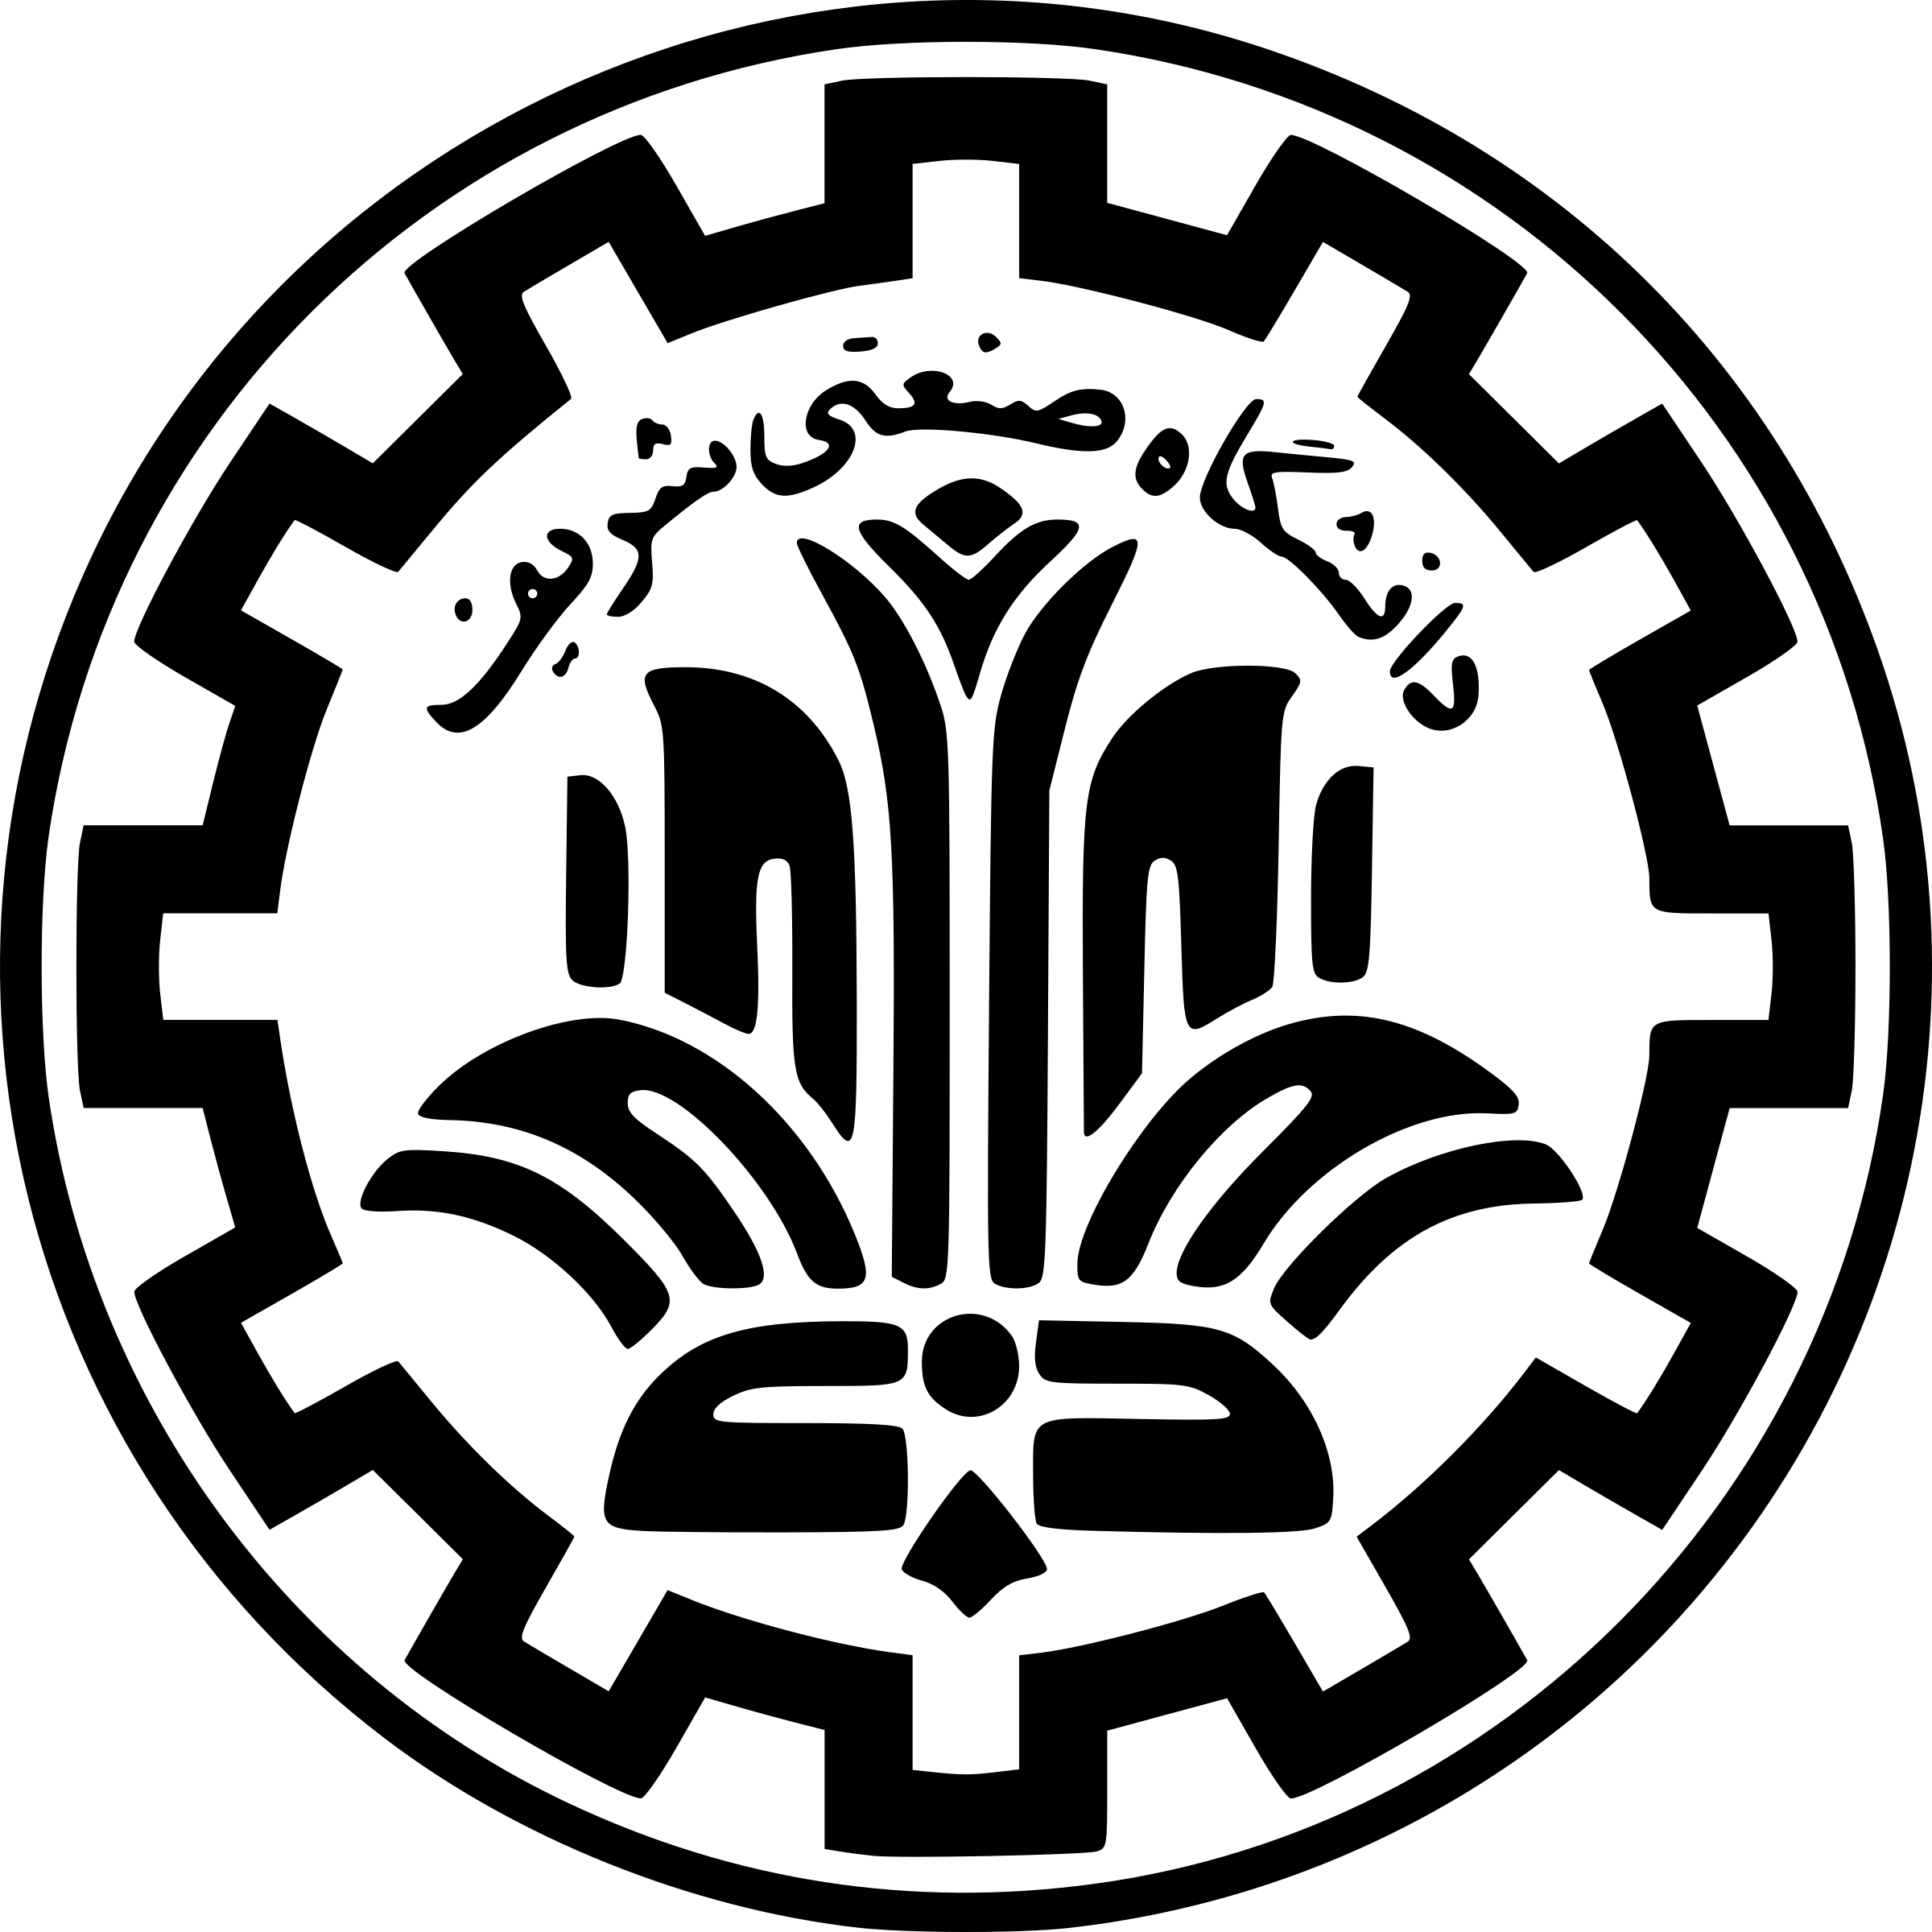
\includegraphics[width=4cm]{sharif.png}\\[1.5cm]
		{\Large\textbf{دانشگاه صنعتی شریف}}\\[0.5cm]
		{\large\textbf{دانشکده‌ٔ مهندسی کامپیوتر}}\\[1.5cm]
		{\Huge\textbf{گزارش کار آزمایشگاه}}\\[0.5cm]
		{\LARGE\textbf{آزمایشگاه سیستم‌های عامل}}\\[2cm]
		
		\textbf{گزارش آزمایش شماره ۱۰}\\
		(آشنایی با درایور‌ها)
		
		\vfill
		\begin{tabular}{rl}
			\textbf{شماره‌ی گروه:} & ۲۰ \\
			\textbf{گروه:} &
			ارشیا یوسف‌نیا (۴۰۱۱۱۰۴۱۵) \\
			& محمدعارف زارع زاده (۴۰۱۱۰۶۰۱۷) \\
			\textbf{استاد درس:} & دکتر بیگی \\
			\textbf{تاریخ:} & تابستان ۱۴۰۴ \\
		\end{tabular}
	\end{titlepage}
	
	% ==============================
	% Persian Ordinal Page Numbering
	% ==============================
	\clearpage
	\setcounter{page}{1}
	\renewcommand{\thepage}{\persianordinalpage}
	
	\tableofcontents
	\clearpage
	\listoffigures
	%\clearpage
	%\listoftables
	
	% ==============================
	% Switch to Persian Digits (۱, ۲, ۳, ...)
	% ==============================
	\clearpage
	\setcounter{page}{1}
	\pagenumbering{arabic}
	\renewcommand{\thepage}{\persianfont\arabic{page}}
	
	
	% ==============================
	% Main Content
	% ==============================
	\section{آزمایش ۱}
	\subsection{نیازمندی‌های اجرا}
	برای ساخت ماژول و بارگذاری و حذف، مراحل زیر را دنبال کنید:
	
	\begin{english}
		\noindent
		\# install required dependencies \\
		sudo apt upgrade \\
		sudo apt install build-essential linux-headers-\$(uname -r) \\
		\# command to build a driver module \\
		make \\
		\# commands to load and remove a driver module \\
		sudo insmode driver.ko \\
		sudo rmmod driver.ko
	\end{english}
	
	\subsection{توضیح کد و روند آزمایش}
	در این بخش یک درایور ساده می‌نویسیم که که صرفا یک پیام برای ما چاپ کند تا از درستی کار خود آگاه شویم. برای نوشتن این درایور اتفاقاتی که باید در هنگام لود شدن و در هنگام خروج انجام شود را مشخص کنیم. در اینجا در هر دو مورد صرفا یک لاگ می‌اندازیم. شکل \ref{img:1} این برنامه را نشان می‌دهد که تابعی که باید هنگام آغاز و خروج فراخوانی شود را مشخص می‌کند و نکاتی مثل توضیح یا لایسنس را هم مشخص می‌کند. در نهایت برای ساخت و کامپایل محتوای \textenglish{Makefile} را مطابق شکل \ref{img:2} پر می‌کنیم تا درایور آماده نصب شود. در شکل \ref{img:3} نتیجه ساخت و نصب درایور مشاهده می‌شود. همچنین با دستور \textenglish{dmesg} لاگ‌ها را بررسی می‌کنیم و پیام‌های خود را پیدا می‌کنیم. همه فایل‌ها به پیوست گزارش ارسال شده است.
	\begin{figure}[H]
		\centering
		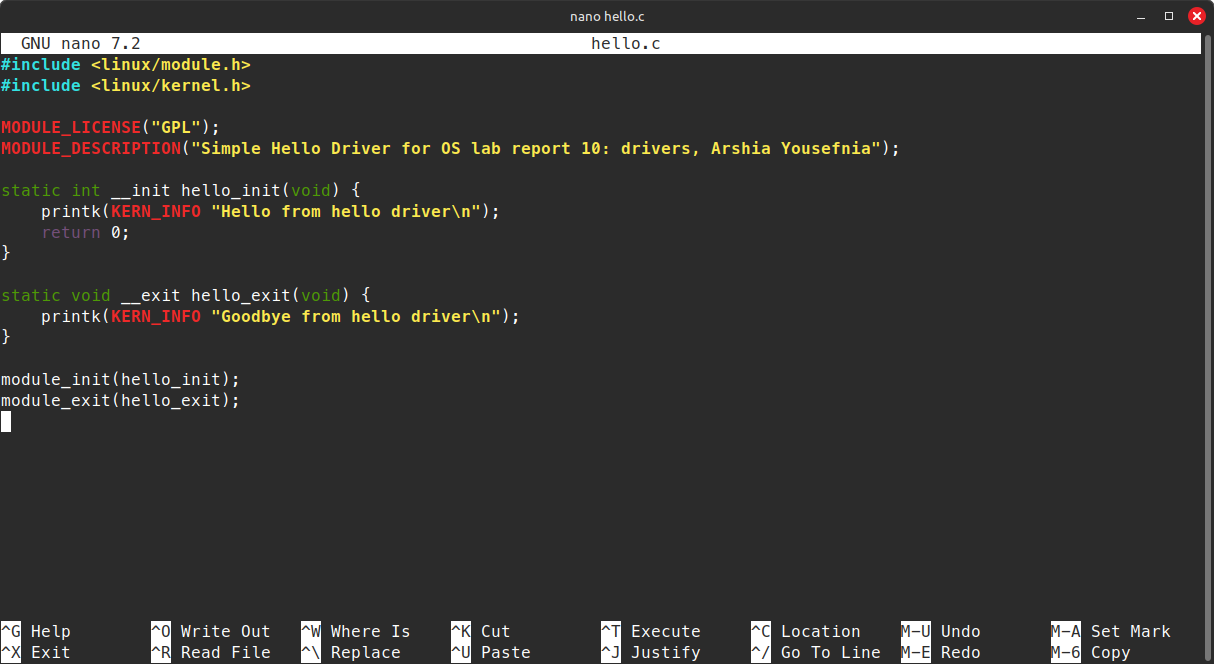
\includegraphics[width=\textwidth]{report10-resources/screenshots/1.png}
		\caption{برنامهٔ درایور آزمایش}
		\label{img:1}
	\end{figure}
	\begin{figure}[H]
		\centering
		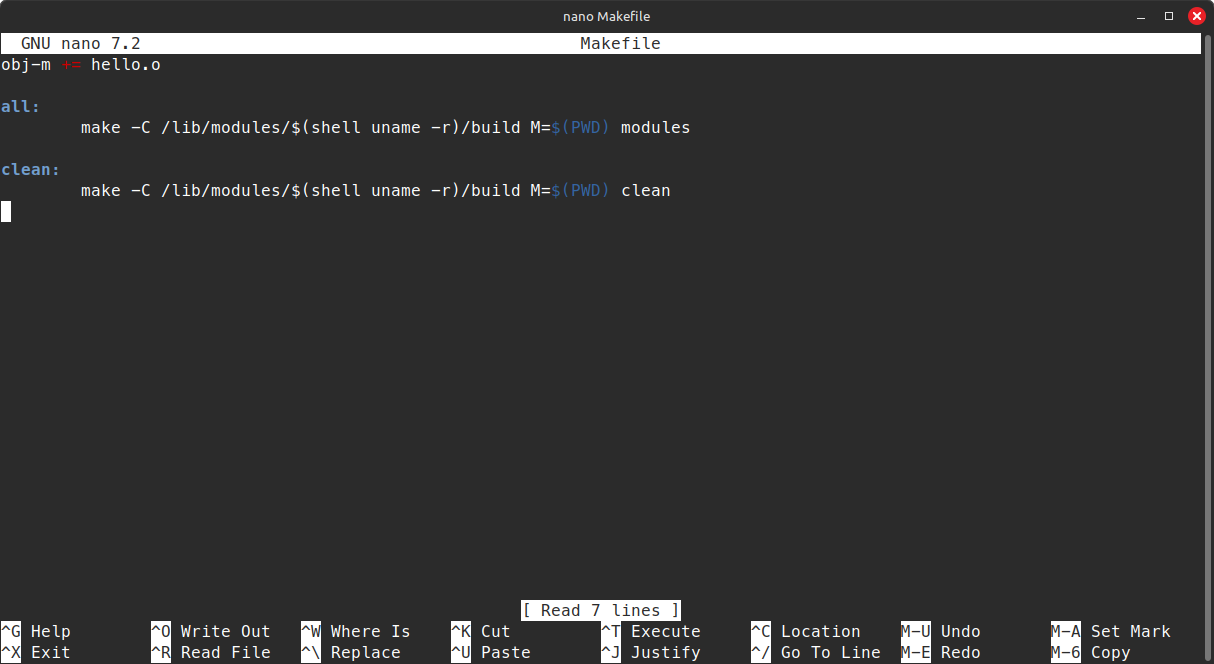
\includegraphics[width=\textwidth]{report10-resources/screenshots/2.png}
		\caption{دستورالعمل ساخت یا \textenglish{Makefile}}
		\label{img:2}
	\end{figure}
	\begin{figure}[H]
		\centering
		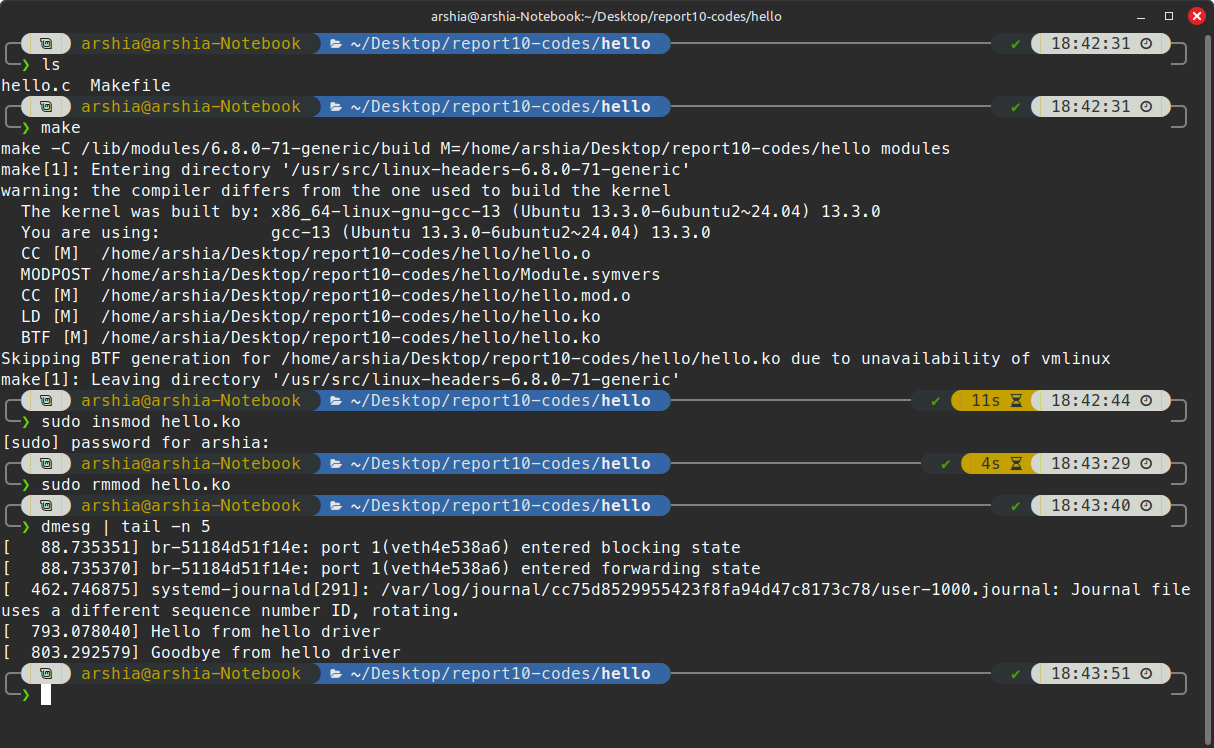
\includegraphics[width=\textwidth]{report10-resources/screenshots/3.png}
		\caption{نتیجهٔ ساخت و استفاده از درایور}
		\label{img:3}
	\end{figure}
	\newpage
	\section{آزمایش ۲}
	\subsection{نیازمندی‌های اجرا}
	مشابه آزمایش قبل:
	
	\begin{english}
		\noindent
		\# install required dependencies \\
		sudo apt upgrade \\
		sudo apt install build-essential linux-headers-\$(uname -r) \\
		\# command to build a driver module \\
		make \\
		\# commands to load and remove a driver module \\
		sudo insmode driver.ko \\
		sudo rmmod driver.ko
	\end{english}
	\subsection{توضیح کد و روند آزمایش}
	در این آزمایش یک درایور می‌نویسیم که با استفاده از \textenglish{netfilter} یک هوک روی ترافیک دستگاه ایجاد کند و از این طریق بتوانیم ترافیک را که با پروتکل \textenglish{ipv4} است رصد کنیم. این هوک لاگ ترافیک را به فایلی که در برنامه مشخص شده می‌ریزد. در آغاز به کار درایور با این هوک را در \textenglish{netfilter} ثبت می‌کنیم و در پایان کار هم آن را برمی‌داریم. این نوع از شنود می‌تواند سربار به سیستم اضافه کند. شکل \ref{img:4} برنامهٔ درایور را نشان می‌دهد که مطابق طرز کار \textenglish{netfilter} یک هوک به آن اضافه کرده‌ایم. در ادامه شکل \ref{img:5} ملزومات ساخت ماژول را نشان می‌دهد. در شکل \ref{img:6} ما درایور را می‌سازیم و آن را لود می‌کنیم، سپس برای تبادل بسته از دستور \textenglish{ping} استفاده می‌کنیم تا ترافیک داشته باشیم. در نهایت درایور را برمیداریم و در شکل \ref{img:7} محتوایات فایلی که برای لاگ بسته‌ها مشخص کردیم را می‌بینیم. برای اطمینان پیام‌های کرنل را هم نگاه می‌کنیم و لاگ‌های نصب و حذف درایور خود را می‌بینیم. همه فایل‌ها به پیوست گزارش ارسال شده است. یک مستند مناسب از \textenglish{netfilter} نیز در \cite{a1} آمده است.
	\begin{figure}[H]
		\centering
		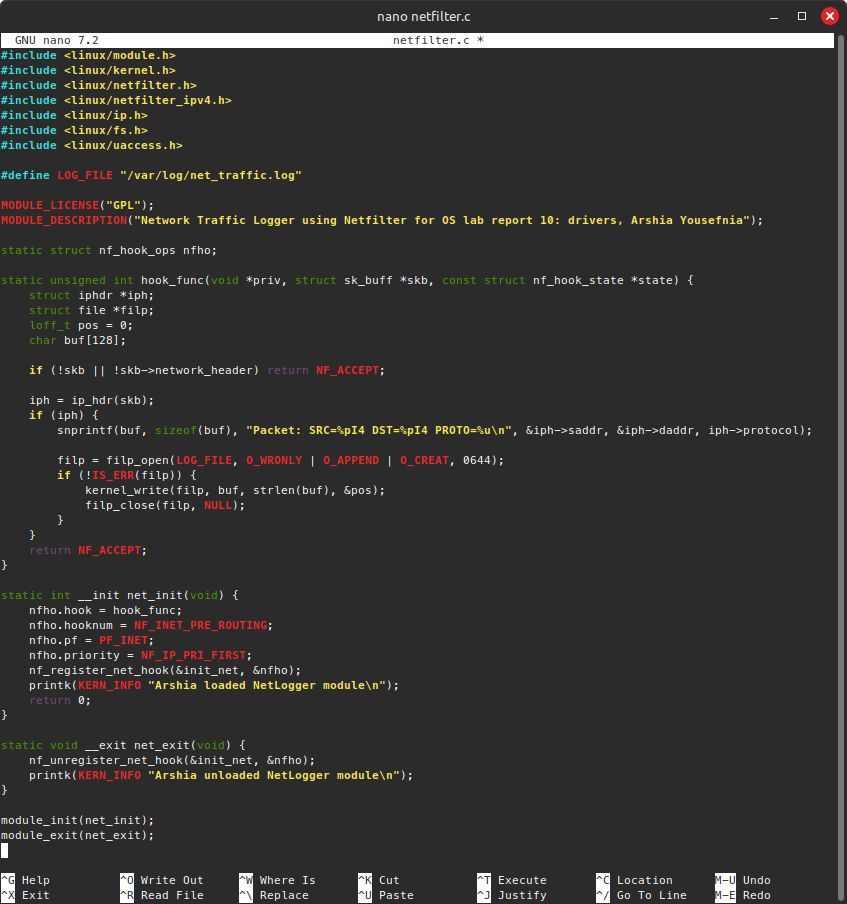
\includegraphics[width=\textwidth]{report10-resources/screenshots/4.png}
		\caption{برنامهٔ درایور آزمایش}
		\label{img:4}
	\end{figure}
	\begin{figure}[H]
		\centering
		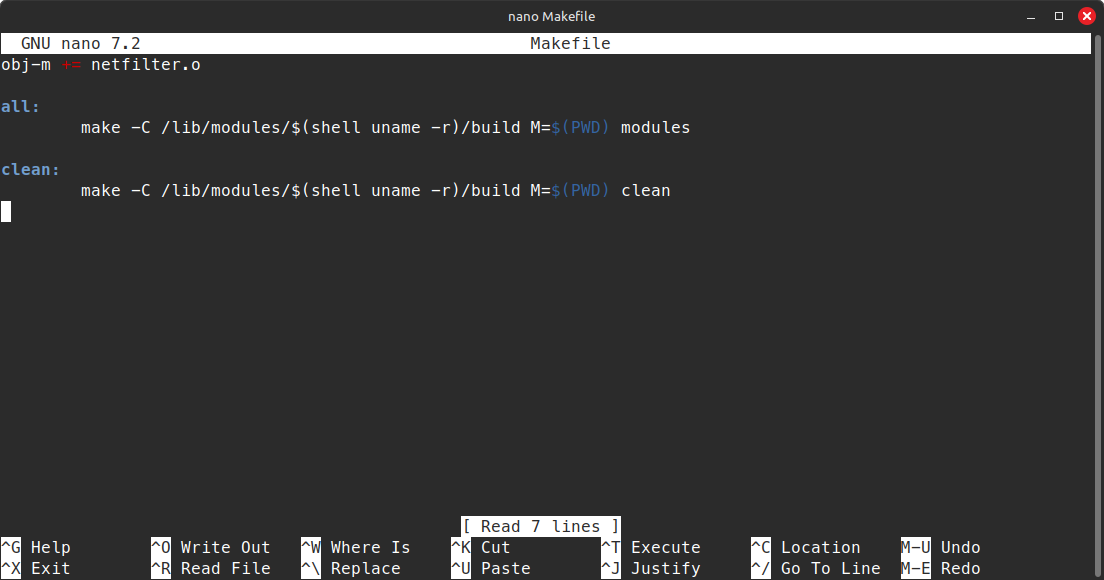
\includegraphics[width=\textwidth]{report10-resources/screenshots/5.png}
		\caption{دستورالعمل ساخت یا \textenglish{Makefile}}
		\label{img:5}
	\end{figure}
	\begin{figure}[H]
		\centering
		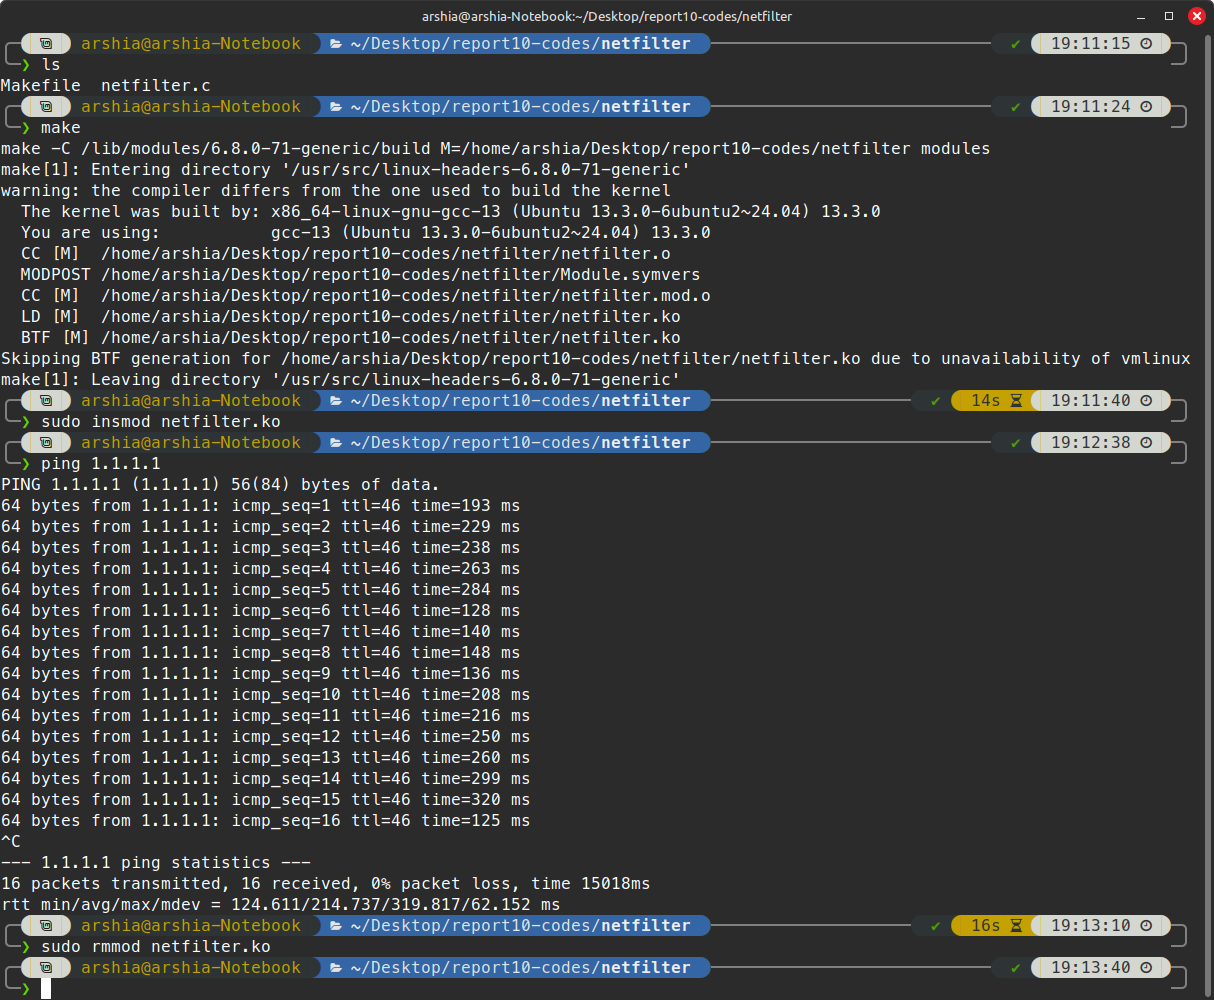
\includegraphics[width=\textwidth]{report10-resources/screenshots/6.png}
		\caption{ساخت و بارگذاری ماژول و تبادل بسته با اینترنت}
		\label{img:6}
	\end{figure}
	\begin{figure}[H]
		\centering
		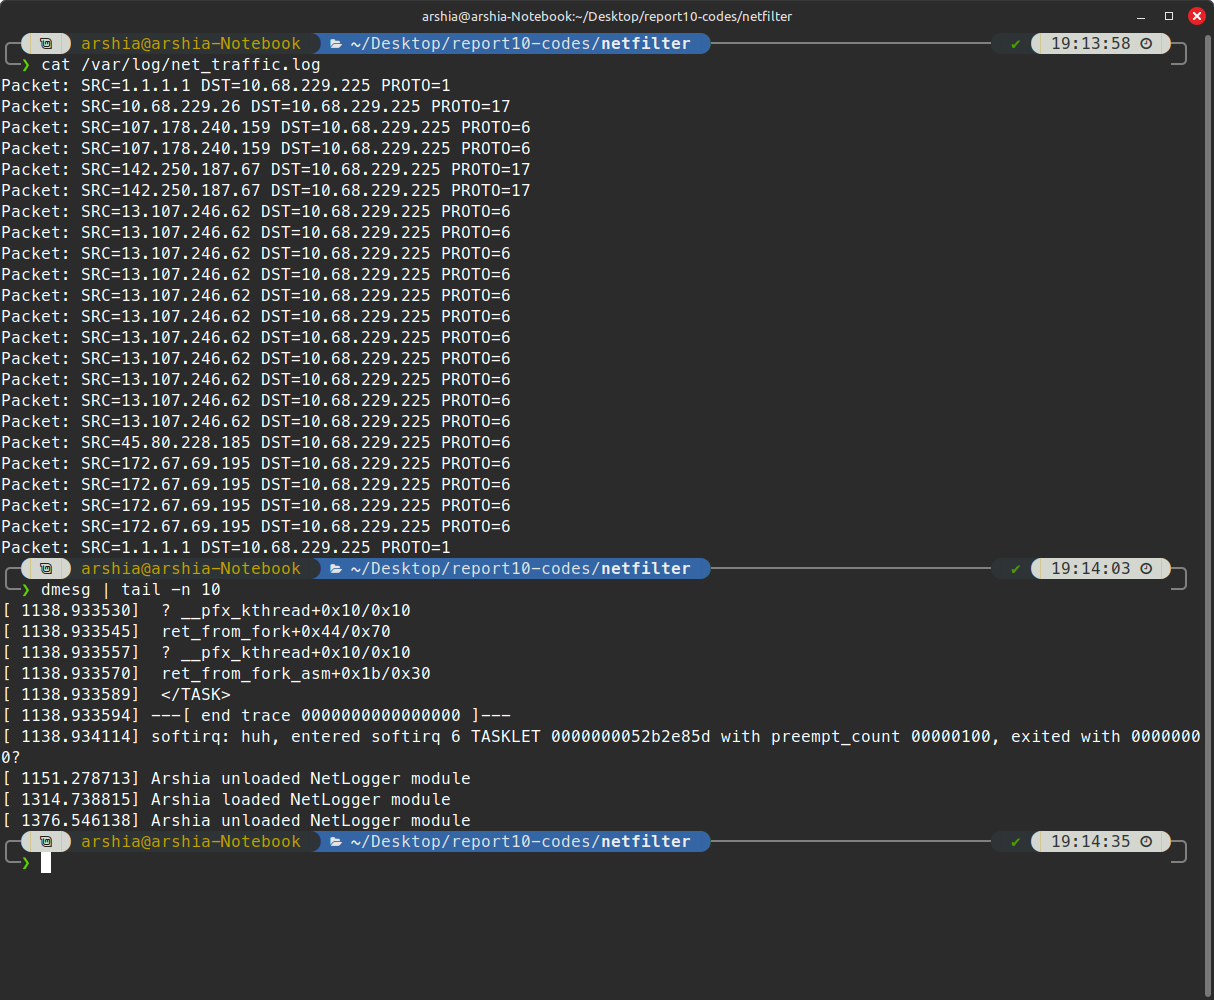
\includegraphics[width=\textwidth]{report10-resources/screenshots/7.png}
		\caption{مشاهده فایل لاگ بسته‌های دیده شده از درایور و پیام‌های کرنل}
		\label{img:7}
	\end{figure}
        
	% ==============================
	% References
	% ==============================
	\newpage
	\begin{LTR}
		\printbibliography[title={مراجع}]
	\end{LTR}

	
\end{document}

